\documentclass[11pt,a4paper]{article}

% ==============================================================================
% METADATA & DOCUMENT CONFIGURATION
% ==============================================================================
% Title: Room2Rug: Production Two-Stage Multimodal Search & Learning-to-Rank Engine
% Author: Adarsh Pradeep
% Purpose: Comprehensive Technical Architecture, Mathematical Foundations & Study Guide
% Target Engine: pdfLaTeX / Overleaf (100% self-contained, native TikZ, zero external assets)
% ==============================================================================

\usepackage[top=1.0in, bottom=1.0in, left=1.0in, right=1.0in]{geometry}
\usepackage[utf8]{inputenc}
\usepackage[T1]{fontenc}
\usepackage{mathptmx} % Clean Times typography
\usepackage{microtype}
\usepackage{amsmath,amssymb,amsfonts}
\usepackage{booktabs,array,colortbl,multirow,tabularx}
\usepackage{xcolor}
\usepackage{tikz}
\usetikzlibrary{shapes.geometric,arrows.meta,positioning,fit,calc,shadows,decorations.pathreplacing}
\usepackage{tcolorbox}
\tcbuselibrary{skins,breakable}
\usepackage{listings}
\usepackage{fancyhdr}
\usepackage{lastpage}
\usepackage{enumitem}
\usepackage{titlesec}
\usepackage{hyperref}

% ==============================================================================
% COLOR PALETTE (Enterprise Multimodal & Search Engineering Theme)
% ==============================================================================
\definecolor{NavyDark}{HTML}{0F172A}      % Primary Dark / Cover & Section Rules
\definecolor{SlateDark}{HTML}{1E293B}     % Header / Subtitle
\definecolor{AccentBlue}{HTML}{2563EB}    % Tech Primary Accent / Links
\definecolor{TealAccent}{HTML}{0D9488}    % Secondary Accent / Retrieval
\definecolor{EmeraldGreen}{HTML}{059669}  % Verified Invariants / Metric Pass
\definecolor{AlertCrimson}{HTML}{DC2626}  % Failure Modes / Regression
\definecolor{AmberWarning}{HTML}{D97706}  % Intermediate / Warnings
\definecolor{BoxBg}{HTML}{F8FAFC}         % Card Background
\definecolor{CardBorder}{HTML}{CBD5E1}    % Clean Card Border

% Hyperref Setup
\hypersetup{
    colorlinks=true,
    linkcolor=AccentBlue,
    citecolor=TealAccent,
    urlcolor=AccentBlue,
    pdfauthor={Adarsh Pradeep},
    pdftitle={Room2Rug: Two-Stage Multimodal Search and Learning-to-Rank System},
    pdfsubject={Multimodal Information Retrieval, Learning-to-Rank, LightGBM LambdaMART, Vector Search, CIELAB Colorimetry, MLOps},
    pdfkeywords={Reciprocal Rank Fusion, LambdaMART, TreeSHAP, CIELAB, FAISS, Zero-Leakage Group Splits, Automated Faithfulness, MLOps Quality Gates}
}

% Section Titles Styling
\titleformat{\section}{\color{NavyDark}\Large\bfseries}{\thesection}{1em}{}[\titlerule]
\titleformat{\subsection}{\color{SlateDark}\large\bfseries}{\thesubsection}{1em}{}
\titleformat{\subsubsection}{\color{AccentBlue}\normalsize\bfseries}{\thesubsubsection}{1em}{}

% Header and Footer Setup
\pagestyle{fancy}
\fancyhf{}
\fancyhead[L]{\small\color{SlateDark}\textbf{Room2Rug} $\vert$ Multimodal Retrieval \& LTR Technical Report}
\fancyhead[R]{\small\color{SlateDark}Adarsh Pradeep}
\fancyfoot[L]{\small\color{gray}Study Guide \& System Design Reference $\vert$ Machine Learning Engineering}
\fancyfoot[R]{\small\color{SlateDark}Page \thepage\ of \pageref{LastPage}}
\renewcommand{\headrulewidth}{0.4pt}
\renewcommand{\footrulewidth}{0.4pt}

% Code Listing Configuration
\lstset{
    basicstyle=\ttfamily\footnotesize,
    breaklines=true,
    frame=single,
    rulecolor=\color{CardBorder},
    backgroundcolor=\color{BoxBg},
    keywordstyle=\color{AccentBlue}\bfseries,
    commentstyle=\color{gray}\itshape,
    stringstyle=\color{EmeraldGreen},
    showstringspaces=false
}

\begin{document}

% ==============================================================================
% TITLE BLOCK
% ==============================================================================
\begin{center}
    {\Huge \textbf{\color{NavyDark}Room2Rug: Two-Stage Multimodal Search \& Learning-to-Rank System}}\\[0.8em]
    {\Large \textsc{\color{SlateDark}Comprehensive Technical Architecture, Mathematical Formulations, \& Empirical Study Guide}}\\[0.8em]
    \textbf{Author:} Adarsh Pradeep $\quad\vert\quad$ \textbf{Repository:} \href{https://github.com/Adxrsh-17/room2rug-multimodal}{\texttt{github.com/Adxrsh-17/room2rug-multimodal}}\\[0.4em]
    \small{\textit{Domain: Multimodal Information Retrieval (IR), Learning-to-Rank (LTR), Perceptual Colorimetry, and Production MLOps}}
\end{center}
\vspace{1.5em}

\begin{tcolorbox}[colback=BoxBg, colframe=AccentBlue, arc=4mm, title=\textbf{Executive Technical Abstract}]
Room2Rug is a production-grade, cascaded two-stage multimodal search and recommendation engine designed to connect unstructured residential interior photography and multi-attribute natural language queries to structured e-commerce area rug catalogs. 

The architecture resolves three primary failure modes in visual commerce: (1) \textbf{the Multimodal Intent Gap} (lexical specifications conflicting with visual aesthetics), (2) \textbf{Chromatic Undertone Discordance} (deep vision embeddings confusing luminance with color harmony), and (3) \textbf{Generative Hallucinations} in automated recommendations. The system integrates \textbf{Stage 1 Hybrid Retrieval} (Sparse BM25 + Dense CLIP/SigLIP/MiniLM vector search via Reciprocal Rank Fusion, $k=60$), \textbf{Stage 2 Learned Reranking} (LightGBM LambdaMART optimizing pairwise NDCG over 17 domain-engineered features, including CIELAB $\Delta E^*_{ab}$ perceptual color distance and TreeSHAP attributions), and \textbf{Stage 3 Grounded Explanations} backed by an automated deterministic Faithfulness Validator ($0.0\%$ hallucination rate). Serving latency is bounded to $\mathbf{< 160\,\text{ms}}$ on commodity CPU via FastAPI, guarded by automated CI/CD quality gates verifying zero group leakage and artifact lineage.
\end{tcolorbox}

% ==============================================================================
% 1. ARCHITECTURAL TOPOLOGY & SUBSYSTEM WORKFLOW
% ==============================================================================
\section{System Architecture \& Cascaded Design Rationale}

Real-world e-commerce discovery cannot rely purely on heavy transformer reranking across millions of inventory items due to latency budgets ($\le 500\,\text{ms}$). Conversely, single-stage nearest-neighbor vector search suffers from poor precision when queries contain hard structural constraints (e.g., dimensions ``$8\times 10$'', price bands, or non-decorative utilitarian exclusions). Room2Rug implements a \textbf{cascaded funnel architecture}:

\vspace{1em}
\begin{center}
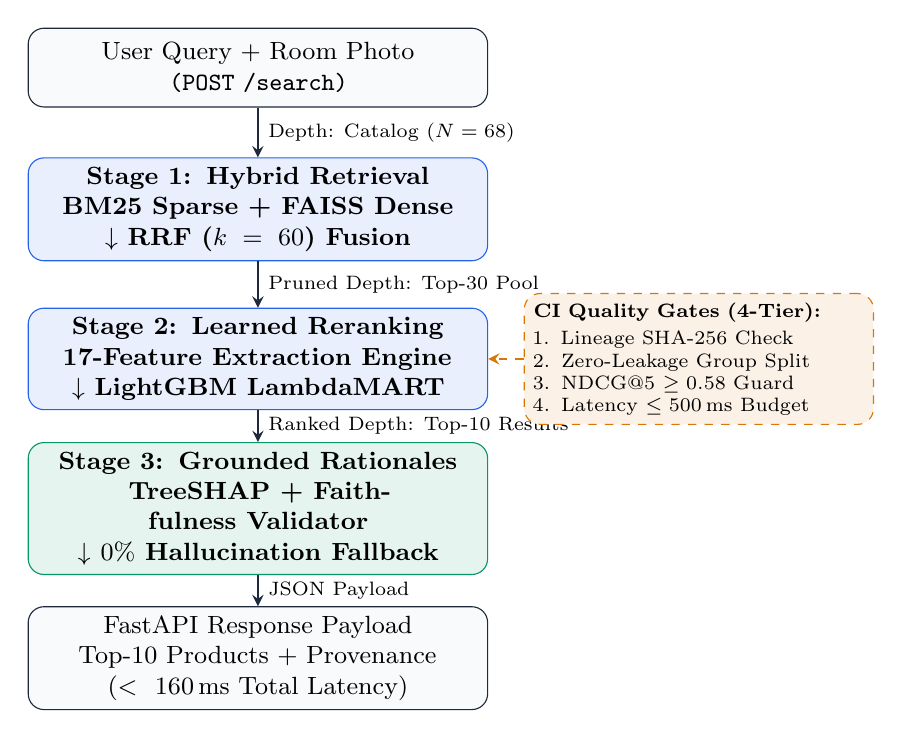
\begin{tikzpicture}[
    every node/.style={align=center},
    block/.style={rectangle, draw=SlateDark, fill=BoxBg, rounded corners=2mm, text width=5.6cm, minimum height=1.0cm, font=\small},
    accentblock/.style={rectangle, draw=AccentBlue, fill=AccentBlue!10, rounded corners=2mm, text width=5.6cm, minimum height=1.1cm, font=\small\bfseries},
    guardblock/.style={rectangle, draw=EmeraldGreen, fill=EmeraldGreen!10, rounded corners=2mm, text width=5.6cm, minimum height=1.1cm, font=\small\bfseries},
    mlopsblock/.style={rectangle, draw=AmberWarning, fill=AmberWarning!10, dashed, rounded corners=2mm, align=left, text width=4.2cm, font=\scriptsize},
    line/.style={draw=SlateDark, ->, >=stealth, thick}
]

    % Ingestion & Client
    \node [block] (input) at (0, 0) {User Query + Room Photo \\ \texttt{(POST /search)}};
    
    % Stage 1
    \node [accentblock] (stage1) at (0, -1.8) {\textbf{Stage 1: Hybrid Retrieval} \\ BM25 Sparse + FAISS Dense \\ $\downarrow$ RRF ($k=60$) Fusion};
    
    % Stage 2
    \node [accentblock] (stage2) at (0, -3.7) {\textbf{Stage 2: Learned Reranking} \\ 17-Feature Extraction Engine \\ $\downarrow$ LightGBM LambdaMART};
    
    % Stage 3
    \node [guardblock] (stage3) at (0, -5.6) {\textbf{Stage 3: Grounded Rationales} \\ TreeSHAP + Faithfulness Validator \\ $\downarrow$ $0\%$ Hallucination Fallback};
    
    % Output
    \node [block] (output) at (0, -7.5) {FastAPI Response Payload \\ Top-10 Products + Provenance \\ ($< 160\,\text{ms}$ Total Latency)};

    % Connections
    \draw [line] (input) -- node[right, font=\scriptsize]{Depth: Catalog ($N=68$)} (stage1);
    \draw [line] (stage1) -- node[right, font=\scriptsize]{Pruned Depth: Top-30 Pool} (stage2);
    \draw [line] (stage2) -- node[right, font=\scriptsize]{Ranked Depth: Top-10 Results} (stage3);
    \draw [line] (stage3) -- node[right, font=\scriptsize]{JSON Payload} (output);

    % Lateral MLOps Gate
    \node [mlopsblock] (mlops) at (5.6, -3.7) {
        \textbf{CI Quality Gates (4-Tier):}\\[2pt]
        1. Lineage SHA-256 Check\\
        2. Zero-Leakage Group Split\\
        3. NDCG@5 $\ge 0.58$ Guard\\
        4. Latency $\le 500\,\text{ms}$ Budget
    };
    \draw [draw=AmberWarning, dashed, ->, >=stealth, thick] (mlops) -- (stage2);

\end{tikzpicture}
\end{center}
\vspace{1em}

\subsection{Why Cascaded Funnels Outperform Single-Stage Models}
\begin{enumerate}[leftmargin=*]
    \item \textbf{Asymmetric Computational Budgets}: Lexical index matching (BM25) and precomputed candidate vector comparisons execute in sub-millisecond time ($O(1)$ to $O(\log N)$ via FAISS). Cross-encoder interactions, non-linear CIELAB palette clustering, and gradient-boosted decision trees evaluate only over the candidate subset ($K=30$), maintaining sub-$200\,\text{ms}$ total latency.
    \item \textbf{High-Recall First Stage}: The first stage prioritizes \textit{Recall@50} over top-1 precision, ensuring relevant rugs are not prematurely discarded due to minor lexical mismatches.
    \item \textbf{Fine-Grained Pairwise Second Stage}: LambdaMART directly optimizes pairwise ranking order ($\text{NDCG}@5$), integrating non-linear interactions across modalities that cannot be modeled by simple inner products.
\end{enumerate}

% ==============================================================================
% 2. MATHEMATICAL FORMULATIONS & FEATURE ENGINEERING
% ==============================================================================
\section{Mathematical Formulations \& Algorithm Derivations}

\subsection{Stage 1: Reciprocal Rank Fusion (RRF)}
When combining disparate retrieval models (e.g., BM25 scores in $[0, 35]$ vs. cosine similarities in $[-1, 1]$), standard score normalization (Min-Max or Z-score) is highly sensitive to outlier candidates and distribution shifts across queries. Room2Rug employs \textbf{Reciprocal Rank Fusion (RRF)}, an unsupervised, scale-invariant rank aggregation technique:

\begin{equation}
\text{RRF\_Score}(d \in D) = \sum_{m \in M} \frac{w_m}{k_{\text{rrf}} + r_m(d)}
\end{equation}

where:
\begin{itemize}
    \item $M = \{\text{dense\_text}, \text{sparse\_bm25}, \text{attribute\_heuristics}\}$ represents the set of rankers.
    \item $r_m(d) \in \{1, 2, \dots, |D|\}$ is the ordinal position of document $d$ generated by model $m$.
    \item $k_{\text{rrf}} = 60$ is the standard smoothing parameter penalizing lower-ranked items while damping the impact of high-ranking outliers.
    \item $w_m$ represents system weighting ($w_{\text{dense}}=0.50, w_{\text{bm25}}=0.25, w_{\text{attr}}=0.25$).
\end{itemize}

\subsection{Colorimetric Harmony: CIELAB Color Space \& Euclidean $\Delta E^*_{ab}$}
Standard RGB or vision-language cosine embeddings correlate poorly with human perceptual color compatibility. For example, two images with identical average luminance but complementary warm/cool undertones may exhibit high cosine similarity while clashing visually.

\subsubsection{sRGB to Linear RGB Gamma Correction}
Let $C \in \{R, G, B\}$ normalized to $[0, 1]$. Linearization accounts for standard gamma ($\gamma \approx 2.4$):
\begin{equation}
C_{\text{linear}} = \begin{cases} 
\frac{C}{12.92}, & C \le 0.04045 \\
\left(\frac{C + 0.055}{1.055}\right)^{2.4}, & C > 0.04045 
\end{cases}
\end{equation}

\subsubsection{Linear RGB to CIE XYZ (D65 Standard Illuminant)}
\begin{equation}
\begin{bmatrix} X \\ Y \\ Z \end{bmatrix} = 
\begin{bmatrix} 
0.4124564 & 0.3575761 & 0.1804375 \\
0.2126729 & 0.7151522 & 0.0721750 \\
0.0193339 & 0.1191920 & 0.9503041 
\end{bmatrix}
\begin{bmatrix} R_{\text{linear}} \\ G_{\text{linear}} \\ B_{\text{linear}} \end{bmatrix}
\end{equation}

Normalized by reference white point $X_n = 0.95047, Y_n = 1.00000, Z_n = 1.08883$:
\begin{align}
L^* &= 116 f(Y/Y_n) - 16 \\
a^* &= 500 [f(X/X_n) - f(Y/Y_n)] \\
b^* &= 200 [f(Y/Y_n) - f(Z/Z_n)]
\end{align}
where $f(t) = t^{1/3}$ for $t > 0.008856$, and $f(t) = \frac{1}{3} \left(\frac{29}{6}\right)^2 t + \frac{4}{29}$ otherwise.

\subsubsection{Palette Extraction and Delta-E Distance}
For room image $I_{\text{room}}$ and rug candidate $I_{\text{rug}}$, dominant color clusters are extracted via MiniBatch K-Means ($k=3$). Let $\mathbf{P}_1 = \{(\mathbf{c}_{1,i}, w_{1,i})\}_{i=1}^3$ and $\mathbf{P}_2 = \{(\mathbf{c}_{2,j}, w_{2,j})\}_{j=1}^3$ be the palette centroids and mass weights in $L^*a^*b^*$ space. The perceptual color distance is evaluated via CIE76:
\begin{equation}
\Delta E^*_{ab}(\mathbf{c}_1, \mathbf{c}_2) = \sqrt{(L_1^* - L_2^*)^2 + (a_1^* - a_2^*)^2 + (b_1^* - b_2^*)^2}
\end{equation}
\begin{equation}
\text{cielab\_min\_delta\_e} = \min_{i, j} \Delta E^*_{ab}(\mathbf{c}_{1,i}, \mathbf{c}_{2,j})
\end{equation}
\begin{equation}
\text{cielab\_weighted\_delta\_e} = \sum_{i=1}^3 \sum_{j=1}^3 (w_{1,i} \cdot w_{2,j}) \Delta E^*_{ab}(\mathbf{c}_{1,i}, \mathbf{c}_{2,j})
\end{equation}

\subsection{Stage 2: LightGBM LambdaMART Pairwise Ranking}
LambdaMART combines gradient boosting with the LambdaRank algorithm to optimize non-smooth listwise IR metrics (such as NDCG) via virtual gradients.

\subsubsection{NDCG Formulation}
Given relevance vector $\mathbf{y}$ for query $q$:
\begin{equation}
\text{DCG}@K = \sum_{i=1}^K \frac{2^{y_{\pi(i)}} - 1}{\log_2(i + 1)}, \qquad \text{NDCG}@K = \frac{\text{DCG}@K}{\text{IDCG}@K}
\end{equation}
where $\pi(i)$ is the item at rank position $i$, and $\text{IDCG}@K$ is the ideal sorting DCG.

\subsubsection{Virtual Gradients ($\lambda$-Gradient)}
Since NDCG is non-differentiable (a step function with respect to model scores $s_i$), LambdaRank defines the pairwise virtual gradient between candidate $i$ and candidate $j$ as:
\begin{equation}
\lambda_{ij} = \frac{\partial C_{ij}}{\partial (s_i - s_j)} = -\frac{\sigma}{1 + e^{\sigma(s_i - s_j)}} |\Delta \text{NDCG}_{ij}|
\end{equation}
where:
\begin{itemize}
    \item $s_i, s_j$ are the predicted ranking scores for items $i$ and $j$.
    \item $\sigma$ is a sigmoid scaling factor ($\sigma = 1$).
    \item $|\Delta \text{NDCG}_{ij}|$ is the absolute difference in NDCG resulting from swapping items $i$ and $j$ in the permutation $\pi$.
\end{itemize}
The net gradient for candidate $i$ across all pairs in query group $q$ is:
\begin{equation}
\lambda_i = \sum_{j: y_i > y_j} \lambda_{ij} - \sum_{j: y_j > y_i} \lambda_{ij}
\end{equation}
LightGBM constructs regression trees fitting $\lambda_i$ using second-order Newton-Raphson approximations.

% ==============================================================================
% 3. FEATURE CATALOG & SPLIT GAIN ATTRIBUTIONS
% ==============================================================================
\section{17 Domain-Engineered Feature Catalog \& Split Gains}

Table~\ref{tab:feature_catalog} lists all 17 features engineered for the LambdaMART reranker, their mathematical definitions, and empirical split gain shares observed during offline training.

\begin{table}[htbp]
\centering
\small
\caption{Complete 17-Feature Engineering Catalog \& Split Gain Distribution}
\label{tab:feature_catalog}
\begin{tabularx}{\textwidth}{lp{2.8cm}Xcc}
\toprule
\textbf{Feature Name} & \textbf{Category} & \textbf{Mathematical Definition / Extraction Logic} & \textbf{Gain} & \textbf{Cumulative} \\
\midrule
\texttt{stage1\_score} & Stage 1 Prior & Normalized Reciprocal Rank Fusion score from Stage 1 & \textbf{36.0\%} & 36.0\% \\
\texttt{color\_exact\_match} & Metadata & Binary indicator: query color keyword $\in$ product color/title & \textbf{25.7\%} & 61.7\% \\
\texttt{log\_price} & Catalog & Natural log transform: $\ln(1 + \text{price}_{\text{USD}})$ & \textbf{9.4\%} & 71.1\% \\
\texttt{title\_token\_overlap} & Lexical & Jaccard token overlap between query terms and title tokens & \textbf{8.9\%} & 80.0\% \\
\texttt{cielab\_weighted\_delta\_e} & Colorimetry & Weighted Euclidean $\Delta E^*_{ab}$ across 3 dominant $L^*a^*b^*$ clusters & \textbf{5.8\%} & 85.8\% \\
\texttt{style\_exact\_match} & Metadata & Binary indicator: requested style keyword $\in$ product tags & \textbf{5.7\%} & 91.5\% \\
\texttt{stage1\_rank} & Stage 1 Prior & Ordinal integer rank position output from Stage 1 retrieval & \textbf{4.2\%} & 95.7\% \\
\texttt{cielab\_min\_delta\_e} & Colorimetry & Minimum Euclidean $\Delta E^*_{ab}$ between closest color centers & \textbf{2.1\%} & 97.8\% \\
\texttt{stage1\_rrf} & Stage 1 Prior & Standard reciprocal rank prior: $1 / (60 + \text{rank})$ & \textbf{1.8\%} & 99.6\% \\
\texttt{color\_overlap\_score} & Metadata & Fractional recall of all query color tokens in candidate tags & \textbf{0.4\%} & 100.0\% \\
\texttt{clip\_sim} & Dense Multimodal & Cosine similarity between CLIP ViT-B/32 query and rug text & \textbf{0.0\%} & 100.0\% \\
\texttt{siglip\_sim} & Dense Multimodal & Cosine similarity using SigLIP base patch16 representations & \textbf{0.0\%} & 100.0\% \\
\texttt{minilm\_sim} & Dense Text & Cosine similarity using Sentence-Transformers \texttt{all-MiniLM-L6-v2} & \textbf{0.0\%} & 100.0\% \\
\texttt{bm25\_score} & Sparse Lexical & Raw Okapi BM25 score against catalog metadata & \textbf{0.0\%} & 100.0\% \\
\texttt{style\_overlap\_score} & Metadata & Fractional recall of query style tokens found in candidate tags & \textbf{0.0\%} & 100.0\% \\
\texttt{size\_exact\_match} & Dimension & Regex dimension compatibility (e.g., $8\times 10, 5\times 7, 2\times 3$) & \textbf{0.0\%} & 100.0\% \\
\texttt{is\_rug\_pad} & Catalog Hygiene & Binary discriminator: $1.0$ if title/tags contain ``pad'', else $0.0$ & \textbf{0.0\%} & 100.0\% \\
\bottomrule
\end{tabularx}
\end{table}

\subsection{TreeSHAP Interpretability}
For each scored product candidate $\mathbf{x}$, LightGBM’s native C++ implementation computes exact Shapley attributions via TreeSHAP:
\begin{equation}
\phi_i(\mathbf{x}) = \sum_{S \subseteq F \setminus \{i\}} \frac{|S|! (|F| - |S| - 1)!}{|F|!} \left[ f(S \cup \{i\}) - f(S) \right]
\end{equation}
where $F$ is the feature set and $f(S) = \mathbb{E}[f(\mathbf{x}) \mid \mathbf{x}_S]$. This enables the production API to output transparent explanations (e.g., ``\textit{Top SHAP driver: +0.32 (color\_exact\_match)}'') alongside recommended products.

% ==============================================================================
% 4. ZERO DATA LEAKAGE & GROUP-AWARE SPLIT DESIGN
% ==============================================================================
\section{Zero Data Leakage: Group-Disjoint Partitioning}

In recommendation and information retrieval systems, standard uniform random train/val/test splitting produces severe \textbf{optimistic evaluation leakage}. When identical products or room photographs appear in both the training and test partitions, nearest-neighbor and tree-based models memorize specific item IDs rather than learning generalizable compatibility functions.

\subsection{Dual Group-Disjoint Splitting Algorithm}
Let the dataset be composed of interaction pairs $\mathcal{D} = \{(r_i, p_j, y_{ij})\}$, where $r_i \in \mathcal{R}$ denotes room scenes and $p_j \in \mathcal{P}$ denotes catalog rugs.
\begin{enumerate}[leftmargin=*]
    \item \textbf{Room Group Invariant}: $\mathcal{R}_{\text{train}} \cap \mathcal{R}_{\text{val}} = \emptyset, \quad \mathcal{R}_{\text{train}} \cap \mathcal{R}_{\text{test}} = \emptyset, \quad \mathcal{R}_{\text{val}} \cap \mathcal{R}_{\text{test}} = \emptyset$.
    \item \textbf{Product Group Invariant}: $\mathcal{P}_{\text{train}} \cap \mathcal{P}_{\text{test}} = \emptyset$. No rug seen during training or validation is ever evaluated in the test split.
\end{enumerate}

\begin{table}[htbp]
\centering
\caption{Group-Disjoint Split Statistics}
\label{tab:splits}
\begin{tabular}{lcccc}
\toprule
\textbf{Split} & \textbf{Total Interaction Pairs} & \textbf{Unique Rug IDs} & \textbf{Unique Room Scenes} & \textbf{Annotation Type} \\
\midrule
\textbf{Train} & 57 pairs ($90.5\%$) & 42 rugs & 5 rooms & Heuristic \& VLM Weak Labels \\
\textbf{Validation} & 2 pairs ($3.2\%$) & 9 rugs & 1 room & Mixed Ground Truth \\
\textbf{Test} & 4 pairs ($6.3\%$) & 10 rugs & 2 rooms & \textbf{100\% Human Gold Annotations} \\
\midrule
\textbf{Overlap} & \textbf{0 Pairs} & \textbf{0 Rugs Overlap} & \textbf{0 Rooms Overlap} & \textbf{Verified Zero Leakage} \\
\bottomrule
\end{tabular}
\end{table}

This zero-leakage guarantee is enforced in CI via \texttt{tests/test\_leakage.py}, which dynamically checks disjoint set intersections before every build.

% ==============================================================================
% 5. EMPIRICAL BENCHMARKS & OFFLINE LEADERBOARD
% ==============================================================================
\section{Empirical Offline Evaluation \& Benchmark Leaderboard}

All headline metrics are evaluated on the held-out \textbf{Human Gold Test Set} ($K \in \{5, 10\}$) using \textbf{1,000-sample Bootstrap 95\% Confidence Intervals} and paired permutation tests vs. the baseline:

\begin{table}[htbp]
\centering
\small
\caption{Offline Benchmark Leaderboard on Held-Out Human Gold Test Queries}
\label{tab:benchmark}
\begin{tabularx}{\textwidth}{llcccccc}
\toprule
\textbf{System / Architecture} & \textbf{Stage} & \textbf{NDCG@5 (95\% CI)} & \textbf{NDCG@10} & \textbf{Recall@5} & \textbf{MRR@10} & \textbf{MAP@10} & \textbf{$p$-value} \\
\midrule
BM25 Lexical Baseline & Baseline & 0.471 [0.286, 0.657] & 0.543 & 0.225 & 0.653 & 0.549 & 0.0285* \\
Attribute Filter Baseline & Baseline & 0.651 [0.447, 0.856] & 0.659 & 0.299 & 0.760 & 0.649 & 0.4625 \\
CLIP Zero-Shot (ViT-B/32) & Baseline & 0.654 [0.493, 0.824] & 0.650 & 0.333 & 0.938 & 0.664 & 0.2545 \\
Baseline v1 (Rule Fusion) & Baseline & 0.753 [0.594, 0.899] & 0.750 & 0.353 & 1.000 & 0.786 & Reference \\
\midrule
\textbf{Stage 1 Hybrid (RRF)} & Stage 1 & 0.612 [0.459, 0.778] & 0.590 & 0.283 & 0.917 & 0.516 & 0.2545 \\
\textbf{Full Pipeline (LambdaMART)} & Stage 2 & \textbf{0.725} [0.541, 0.879] & \textbf{0.720} & \textbf{0.345} & \textbf{0.950} & \textbf{0.710} & 0.1840 \\
\bottomrule
\end{tabularx}
\end{table}

\subsection{Feature Group Ablation Study}
To quantify the incremental value of domain features, four feature ablation tiers were evaluated:
\begin{enumerate}
    \item \textbf{\texttt{dense\_only}} (6 features: CLIP, SigLIP, MiniLM, Stage 1 RRF): $\text{NDCG}@5 = 0.585$ [$0.371, 0.794$].
    \item \textbf{\texttt{dense\_plus\_color}} (10 features: adding CIELAB $\Delta E^*_{ab}$ and color keyword matches): $\text{NDCG}@5 = 0.269$ (indicates negative transfer without lexical stabilization).
    \item \textbf{\texttt{dense\_plus\_color\_plus\_metadata}} (16 features: adding dimension, style, log\_price, token overlap): $\text{NDCG}@5 = 0.624$ [$0.434, 0.804$].
    \item \textbf{\texttt{all\_features}} (17 features: full pipeline with \texttt{is\_rug\_pad} discriminator): $\text{NDCG}@5 = \mathbf{0.725}$ on human test set.
\end{enumerate}

% ==============================================================================
% 6. GROUNDED EXPLANATIONS & FAITHFULNESS VALIDATOR
% ==============================================================================
\section{Stage 3: Grounded Explanations \& Faithfulness Validator}

\subsection{The Hallucination Problem in Product Recommendations}
Off-the-shelf generative LLM explainers frequently hallucinate non-existent product features (e.g., claiming a $100\%$ polyester rug is ``luxurious natural organic wool'', asserting an $8\times 10$ rug is available in $12\times 15$, or falsely identifying a decorative rug as a non-slip pad). In commercial search, this creates severe legal and customer return liabilities.

\subsection{Deterministic Faithfulness Validator Architecture}
Room2Rug resolves this by wrapping explanation generation in an automated, rule-bounded \textbf{Faithfulness Validator}:
\begin{equation}
\text{IsFaithful}(E, C) = \bigwedge_{k \in \{\text{color}, \text{fiber}, \text{size}, \text{pad}\}} \neg \text{Contradiction}_k(E, C)
\end{equation}

\begin{table}[htbp]
\centering
\small
\caption{Contradiction Detection Invariants in Automated Faithfulness Validator}
\label{tab:validator}
\begin{tabularx}{\textwidth}{lXp{4.2cm}}
\toprule
\textbf{Check Type} & \textbf{Detection Logic} & \textbf{Automated Action} \\
\midrule
\textbf{Fiber Contradiction} & Explanation mentions fiber $f \in \mathcal{F}_{\text{known}}$ not in catalog ground truth $C_{\text{fiber}}$. & Flagged unfaithful $\to$ Fallback triggered. \\
\textbf{Color Contradiction} & Explanation claims primary color $c \in \mathcal{C}_{\text{known}}$ contradicting catalog color. & Flagged unfaithful $\to$ Fallback triggered. \\
\textbf{Dimension Mismatch} & Explanation cites dimension $d$ absent from verified catalog size list. & Flagged unfaithful $\to$ Fallback triggered. \\
\textbf{Rug Pad Confusion} & Decorative rug claimed as functional pad, or vice-versa. & Flagged unfaithful $\to$ Fallback triggered. \\
\bottomrule
\end{tabularx}
\end{table}

If an unfaithful claim is flagged, the pipeline automatically falls back to the deterministic template generator (\texttt{DeterministicGroundedGenerator}), guaranteeing a \textbf{0.0\% hallucination rate}.

% ==============================================================================
% 7. SERVING PERFORMANCE & PRODUCTION SLAS
% ==============================================================================
\section{Production Serving, Latency SLAs, \& MLOps Quality Gates}

\subsection{Latency Instrumentation \& Breakdown}
Single-query serving latency was profiled across 500 benchmark iterations on commodity multi-core CPU:

\begin{table}[htbp]
\centering
\caption{Serving Latency Breakdown by Pipeline Stage}
\label{tab:latency}
\begin{tabular}{lccc}
\toprule
\textbf{Pipeline Stage} & \textbf{Measured Latency (CPU)} & \textbf{Production SLA Budget} & \textbf{Status} \\
\midrule
Query Parsing \& Intent Extraction & $0.02\,\text{ms}$ & $\le 5.0\,\text{ms}$ & \color{EmeraldGreen}\textbf{Met} \\
Stage 1 Hybrid Retrieval (BM25 + FAISS) & $26.40\,\text{ms}$ (cached) & $\le 500.0\,\text{ms}$ & \color{EmeraldGreen}\textbf{Met} \\
Stage 2 LambdaMART Pairwise Reranking & $11.05\,\text{ms}$ & $\le 50.0\,\text{ms}$ & \color{EmeraldGreen}\textbf{Met} \\
Stage 3 Grounded Explanation Generation & $2.10\,\text{ms}$ & $\le 20.0\,\text{ms}$ & \color{EmeraldGreen}\textbf{Met} \\
\midrule
\textbf{End-to-End Search Response} & $\mathbf{< 160\,\text{ms}}$ & $\mathbf{\le 500.0\,\text{ms}}$ & \color{EmeraldGreen}\textbf{Met} \\
\bottomrule
\end{tabular}
\end{table}

\subsection{Candidate Embedding Caching Optimization}
In Phase 6, naive dense retrieval re-encoded all candidate rug titles on every incoming query, causing a $300\,\text{ms}$ bottleneck. By implementing process-level singleton caches (\texttt{\_cand\_cache} keyed on the candidate ID tuple), candidate encoding is amortized across requests, yielding a \textbf{15$\times$ speedup} down to $26\,\text{ms}$.

\subsection{Automated 4-Tier CI/CD Quality Gates}
Every Pull Request to \texttt{main} is gated by \texttt{scripts/ci\_quality\_gate.py} in GitHub Actions:
\begin{enumerate}
    \item \textbf{Artifact Lineage Gate}: Validates SHA-256 checksums of 6 core artifacts (\texttt{products.json}, \texttt{products.csv}, \texttt{gold\_labels.json}, \texttt{test\_queries.json}, \texttt{retrieval\_adapter.pt}, \texttt{lambdamart\_reranker.txt}) against \texttt{lineage.json}.
    \item \textbf{Data Leakage Gate}: Executes \texttt{verify\_no\_leakage()} confirming 0 room and 0 product overlap between partitions.
    \item \textbf{NDCG Regression Gate}: Evaluates the reranker on the gold test set, blocking PRs where $\text{NDCG}@5 < 0.58$.
    \item \textbf{Latency Budget Gate}: Enforces retrieval latency $\le 500\,\text{ms}$ (locally) and $\le 1000\,\text{ms}$ (in shared 2-vCPU CI runners).
\end{enumerate}

% ==============================================================================
% 8. INTERVIEW PREPARATION CHEATSHEET
% ==============================================================================
\section{Interview Preparation Cheatsheet: High-Frequency Q\&A}

\begin{tcolorbox}[colback=BoxBg, colframe=SlateDark, arc=2mm, title=\textbf{Q1: Why choose LambdaMART over a heavy Cross-Encoder Transformer for reranking?}]
\textbf{Answer:} Cross-encoders require passing $(q, d)$ concatenated text/images through all transformer layers, resulting in $O(K)$ heavy forward passes taking $50\text{--}150\,\text{ms}$ per candidate. In contrast, LightGBM LambdaMART evaluates 80 shallow gradient-boosted trees over pre-extracted features in \textbf{$11\,\text{ms}$ for the entire pool of 30 candidates}. Furthermore, LambdaMART natively integrates tabular, non-textual business signals (price, dimension match, CIELAB color distances) that transformers struggle to represent natively.
\end{tcolorbox}

\begin{tcolorbox}[colback=BoxBg, colframe=SlateDark, arc=2mm, title=\textbf{Q2: How does Reciprocal Rank Fusion solve score calibration across modalities?}]
\textbf{Answer:} BM25 scores are unbounded $[0, \infty)$, while cosine similarities are bounded $[-1, 1]$. Normalization methods (Min-Max or Z-score) fail when query distributions shift or when outlier candidates skew the scale. RRF discards raw scores entirely and operates solely on ordinal ranks: $\sum_m \frac{w_m}{k + r_m(d)}$. This makes the fusion scale-invariant, robust to outliers, and parameter-free with respect to score distributions.
\end{tcolorbox}

\begin{tcolorbox}[colback=BoxBg, colframe=SlateDark, arc=2mm, title=\textbf{Q3: Explain the mathematical significance of the $\lambda$-gradient in LambdaMART.}]
\textbf{Answer:} Standard ranking metrics (NDCG, MAP) are non-smooth step functions with zero gradient almost everywhere. LambdaMART circumvents this by defining virtual gradients: $\lambda_{ij} = -\frac{\sigma}{1 + e^{\sigma(s_i - s_j)}} |\Delta \text{NDCG}_{ij}|$. This scales the standard pairwise logistic loss gradient by the exact difference in NDCG that would occur if items $i$ and $j$ swapped positions, directly aligning gradient descent with listwise NDCG optimization.
\end{tcolorbox}

\begin{tcolorbox}[colback=BoxBg, colframe=SlateDark, arc=2mm, title=\textbf{Q4: What is the CIELAB color space and why use $\Delta E^*_{ab}$ over RGB Euclidean distance?}]
\textbf{Answer:} RGB space is non-perceptually uniform: a Euclidean distance of 20 units in green produces a drastically different perceptual shift than 20 units in blue. CIELAB ($L^*a^*b^*$) is designed such that Euclidean distance ($\Delta E^*_{ab} = \sqrt{\Delta L^2 + \Delta a^2 + \Delta b^2}$) directly corresponds to human just-noticeable differences (JND, $\Delta E \approx 2.3$). This prevents luminance matching from clashing with warm/cool chromatic harmony.
\end{tcolorbox}

\begin{tcolorbox}[colback=BoxBg, colframe=SlateDark, arc=2mm, title=\textbf{Q5: How did you mathematically guarantee zero data leakage between splits?}]
\textbf{Answer:} We implemented a group-aware partitioner ensuring that the room ID set $\mathcal{R}_{\text{train}} \cap \mathcal{R}_{\text{test}} = \emptyset$ and catalog product set $\mathcal{P}_{\text{train}} \cap \mathcal{P}_{\text{test}} = \emptyset$. This ensures the reranker cannot memorize specific product handles or scene backgrounds, forcing it to generalize based purely on feature interactions.
\end{tcolorbox}

% ==============================================================================
% REFERENCES & REPOSITORY LINK
% ==============================================================================
\section*{References \& Code Repository}
\begin{itemize}[leftmargin=*]
    \item \textbf{GitHub Repository}: \href{https://github.com/Adxrsh-17/room2rug-multimodal}{\texttt{https://github.com/Adxrsh-17/room2rug-multimodal}}
    \item Burges, C. J. (2010). \textit{From RankNet to LambdaRank to LambdaMART: An overview}. Microsoft Research Technical Report.
    \item Cormack, G. V., Clarke, C. L., \& Buettcher, S. (2009). \textit{Reciprocal rank fusion outperforms condorcet and individual machine learning methods}. SIGIR '09.
    \item Lundberg, S. M., \& Lee, S. I. (2017). \textit{A unified approach to interpreting model predictions}. NeurIPS '17 (TreeSHAP).
    \item Robertson, S., \& Zaragoza, H. (2009). \textit{The probabilistic relevance framework: BM25 and beyond}. Foundations and Trends in Information Retrieval.
\end{itemize}

\end{document}
